\documentclass[aspectratio=169]{beamer}
\usepackage{graphicx}
\usepackage{listings}
\lstset{
    basicstyle=\ttfamily
    }
\usepackage{hyperref}
\usetheme{metropolis}
\title{How to use \ttfamily{poetry}}
\institute{Engineers for Exploration, UC San Diego}
\logo{
\includegraphics[height=.65cm,keepaspectratio]{e4e_logo_350x136.png}}
\setbeamertemplate{caption}[numbered]
\date{November 28, 2023}
\begin{document}
\maketitle
\begin{frame}{Obligatory XKCD}
    \centering
    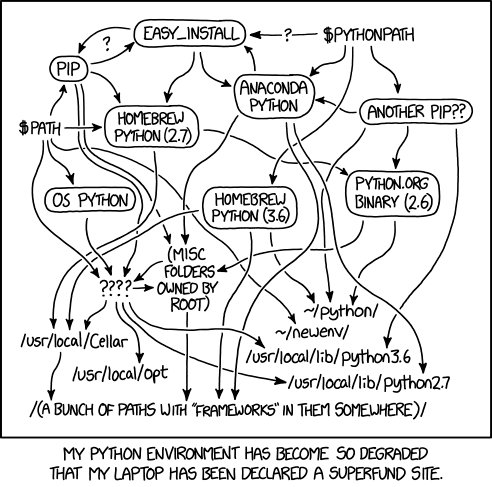
\includegraphics[width=\textwidth,height=0.8\textheight,keepaspectratio]{xkcd_1987_python_environment.png} \footnote{\url{https://xkcd.com/1987}}
\end{frame}
\begin{frame}{Fundamentals: What are Python Packages?}
    \begin{itemize}
        \item Collection of redistributable Python code
        \item Package metadata: PEP 518, PEP 621
    \end{itemize}
    \centering
    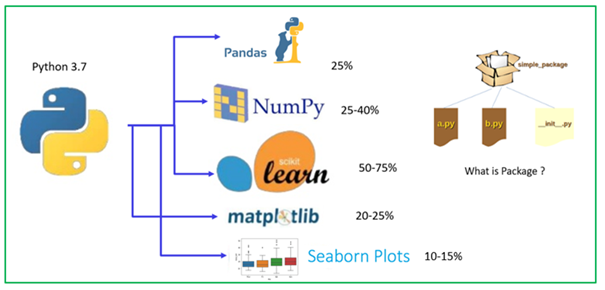
\includegraphics[width=\textwidth,height=0.6\textheight,keepaspectratio]{python_packages.png} \footnote{\url{https://www.analyticsvidhya.com/blog/2021/02/key-python-packages-for-data-science/}}
\end{frame}
\begin{frame}{Fundamentals: What are Package Managers?}
    \begin{itemize}
        \item Package Installation
        \item Package Dependency Resolution
        \item Examples:
        \begin{itemize}
            \item \lstinline!conda!
            \item \lstinline!pip!
            \item \lstinline!pipenv!
            \item \lstinline!poetry!
        \end{itemize}
    \end{itemize}
\end{frame}
\begin{frame}{Package Dependency Management}
    \centering
    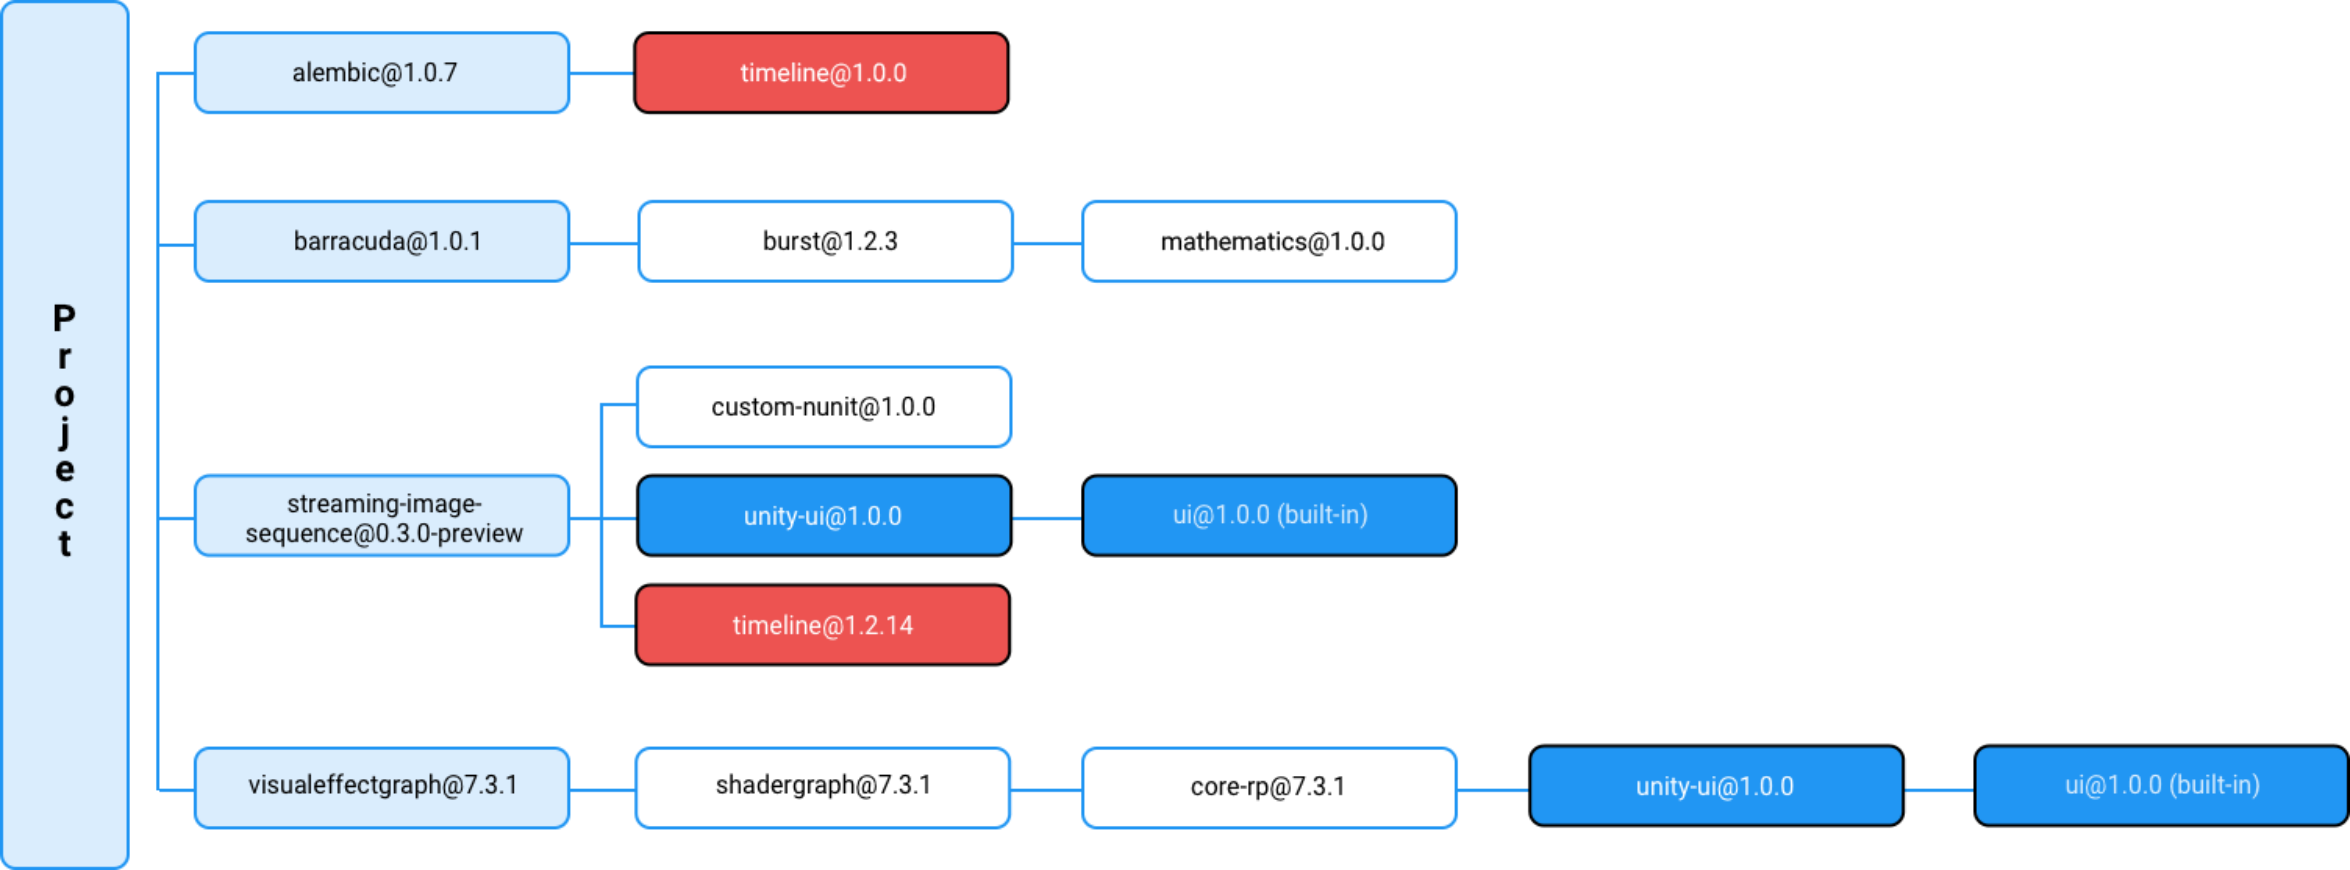
\includegraphics[width=\textwidth,height=0.8\textheight,keepaspectratio]{dependency_resolution.png} \footnote{\url{https://docs.unity3d.com/Manual/upm-conflicts.html}}
\end{frame}
\begin{frame}{Fundamentals: What are Virtual Environments?}
    \begin{itemize}
        \item Isolated execution and configuration contexts
        \item Isolated packages
    \end{itemize}
    \centering
    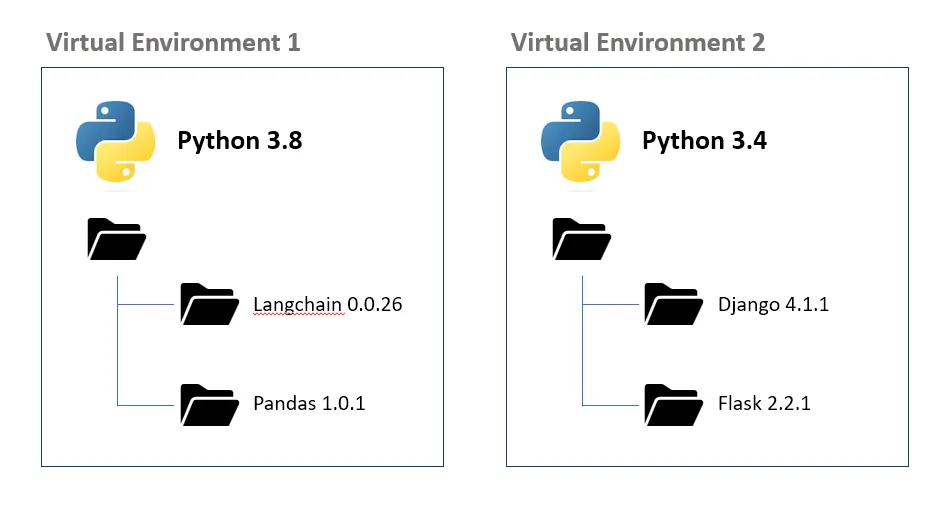
\includegraphics[width=\textwidth,height=0.55\textheight,keepaspectratio]{python_venv.png} \footnote{\url{https://medium.com/@TejasEkawade/installing-python-virtual-environments-cb865c3147a7}}
\end{frame}
\begin{frame}{What else do we want in packages?}
    \begin{itemize}
        \item Authors
        \item Contact info
        \item License info
        \item Version info
        \item Entry points
        \item Dependencies
        \item Development tools
    \end{itemize}
\end{frame}
\begin{frame}{Python Standards}
    \begin{itemize}
        \item \lstinline!requirements.txt!, \lstinline!setup.py!, and \lstinline!setup.cfg! died a long time ago
        \item Use modern build tools
        \item \lstinline!pyproject.toml!
    \end{itemize}
\end{frame}
\begin{frame}{Poetry}
    \begin{itemize}
        \item Package manager
        \item Environment manager
        \item Lockable packages
        \item Mostly accepted by Python community
        \item \url{https://python-poetry.org/}
    \end{itemize}
\end{frame}
\begin{frame}{Practical Example}
    \begin{itemize}
        \item \url{https://github.com/UCSD-E4E/PyHa.git}
        \item Use \lstinline!origin/poetry\_demo!
    \end{itemize}
\end{frame}
\begin{frame}{Which dependencies to add?}
    \centering
    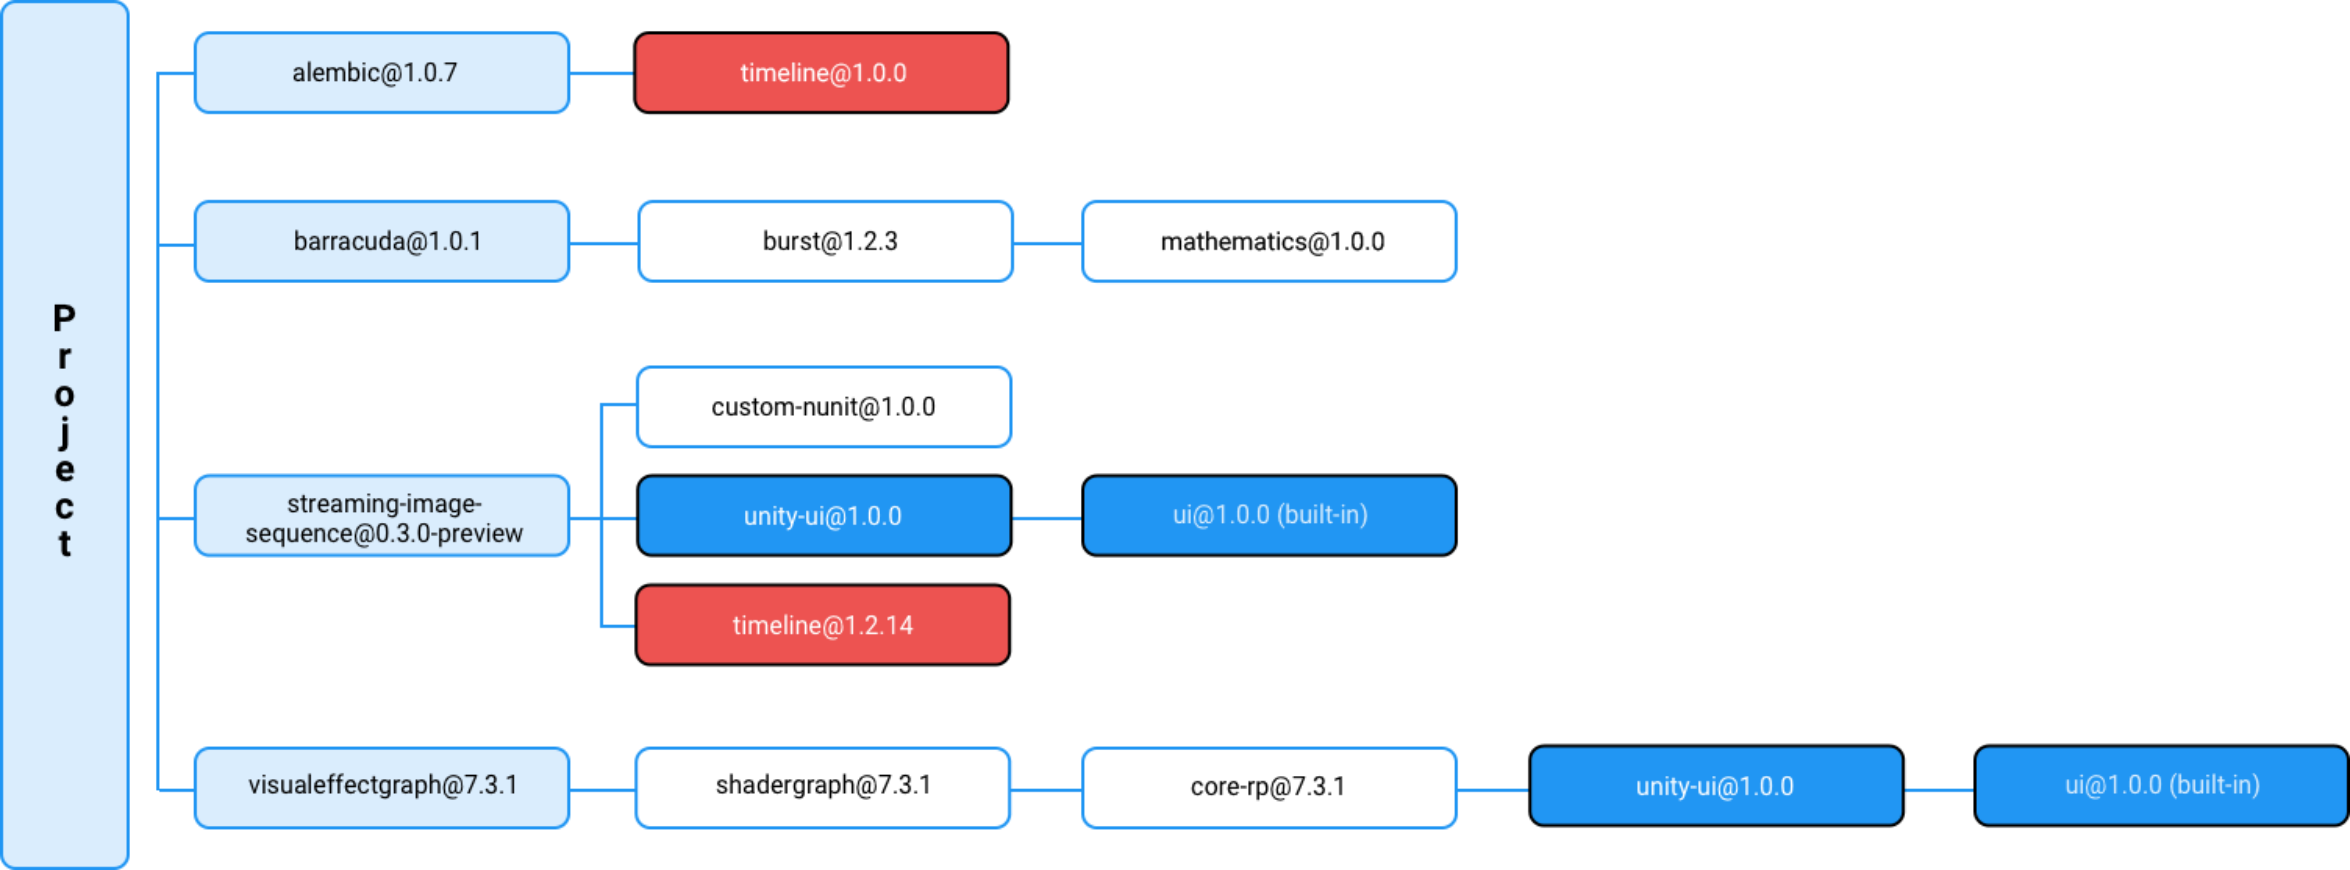
\includegraphics[width=\textwidth,height=0.8\textheight,keepaspectratio]{dependency_resolution.png} \footnote{\url{https://docs.unity3d.com/Manual/upm-conflicts.html}}
\end{frame}
\begin{frame}{Defining dependencies}
    \begin{itemize}
        \item \url{https://python-poetry.org/docs/dependency-specification/}
        \item Semantic Versioning is ideal
        \item But it depends!
        \item General philosophy - err on requiring manual intervention later
    \end{itemize}
\end{frame}
\begin{frame}{Using Poetry with \protect\lstinline!conda!}
    \begin{itemize}
        \item \lstinline!conda! doesn't provide lockfiles!
        \item Introducing \lstinline!conda-lock! (\url{https://pypi.org/project/conda-lock/})
        \item Only if you need \lstinline!conda! only packages, otherwise, use vanilla \lstinline!poetry!
        \item \lstinline!environment.yml! only contains \lstinline!conda! only packages and \lstinline!poetry!
        \item \lstinline!conda-lock -f environment.yml -p osx-64 -p linux-64 -p win-64! to create OS-specific lockfiles
        \item \lstinline!conda create -f conda-[os].lock! to create \lstinline!conda! environment
        \item \lstinline!conda activate! to activate environment
        \item \lstinline!poetry install! to install \lstinline!poetry! lockfile
    \end{itemize}
\end{frame}
\begin{frame}{Additional tools to use with Poetry}
    \begin{itemize}
        \item \lstinline!semantic_release!
    \end{itemize}
\end{frame}
\end{document}